\section{Motor Friction Estimation}
\label{sec:motor_friction_estimation}

This section details the estimation of parameters for the motor friction models of the hip and knee motors. The motors serve as pivot points for pendulums consisting of aluminum rods attached to the motor shafts with ballast masses. The pendulums are released from a horizontal position, and their angular velocity and acceleration are measured. These measurements facilitate the estimation of motor friction coefficients using linear regression. The experimental setup for both motors is depicted in Figure \ref{fig:results:motor_friction_estimation:pendulum_setup}.

\subsection{Friction model}
We adopt a linear friction model as described in section \ref{sec:gear_transmission_friction_model}, incorporating both viscous and Coulomb friction, to accurately fit the observed data. To avoid numerical solver issues from the discontinuity at zero velocity introduced by the Coulomb friction, we used a tanh function to smooth the transition between positive and negative Coulomb friction, expressed as:

\begin{equation}
\label{eq:friction_model}
\tau_{\text{friction}} = b_v \dot{\theta} + b_c \tanh( \dot{\theta} / k)
\end{equation}

where \(k = 0.001\) controls the smoothness of the transitions, maintaining realism while avoiding numerical solver issues.

\subsection{Pendulum Modeling}
The pendulum used in the motor friction tests consists of an aluminum rod of length \( l_{\text{arm}} = 0.21 \) meters and a ballast mass \( m_{\text{ballast}} = 0.301 \) kg with radius \( r_{\text{ballast}} = 0.03 \) meters attached at a distance \( d_{\text{ballast}} = 0.20 \) meters from the pivot. The total mass of the arm is \( m_{\text{arm}} = 0.034 \) kg. The pendulum is modeled as a rigid body rotating about the motor shaft with a total moment of inertia \( I \) composed of the arm inertia \( I_{\text{arm}} \) and ballast inertia \( I_{\text{ballast}} \). The arm is approximated as a thin rod, and the ballast as a disk, both with uniform density. Their inertias are calculated using the parallel axis theorem:

\[
I_{\text{arm}} = \frac{1}{12} m_{\text{arm}} l_{\text{arm}}^2 + m_{\text{arm}} \left(\frac{l_{\text{arm}}}{2}\right)^2
\]

\[
I_{\text{ballast}} = \frac{1}{2} m_{\text{ballast}} r_{\text{ballast}}^2 + m_{\text{ballast}} d_{\text{ballast}}^2
\]

\[
I = I_{\text{arm}} + I_{\text{ballast}}
\]

The torque due to gravity consists of contributions from both the arm and ballast mass:

\[
\tau_{\text{gravity,arm}} = m_{\text{arm}} \frac{l_{\text{arm}}}{2} g \sin(\theta)
\]

\[
\tau_{\text{gravity,ballast}} = m_{\text{ballast}} d_{\text{ballast}} g \sin(\theta)
\]

\[
\tau_{\text{gravity}} = \tau_{\text{gravity,arm}} + \tau_{\text{gravity,ballast}}
\]

The equations of motion, accounting for both viscous and Coulomb friction, are:

\[
I \ddot{\theta} + b_v \dot{\theta} + b_c \, \text{sign}(\dot{\theta}) + \tau_{\text{gravity}} = 0
\]

where:
\begin{itemize}
    \item \( \theta \) is the angular displacement (positive counterclockwise, zero at vertical down position)
    \item \( \dot{\theta} \) and \( \ddot{\theta} \) are the angular velocity and acceleration, respectively
    \item \( b_v \) is the viscous damping coefficient
    \item \( b_c \) is the Coulomb damping coefficient
    \item \( g = 9.81 \, \text{m/s}^2 \) is the acceleration due to gravity
\end{itemize}

\subsection{Data Acquisition}
Pendulum angles \(\theta\) were sampled by manually annotating video frames at 60 Hz using the Tracker program \cite{tracker}. 

The angular velocity \(\dot{\theta}\) and acceleration \(\ddot{\theta}\) are computed using centered finite differences:

\[
\dot{\theta}_i = \frac{\theta_{i+1} - \theta_{i-1}}{2\Delta t}
\]

\[
\ddot{\theta}_i = \frac{\theta_{i+1} - 2\theta_i + \theta_{i-1}}{(\Delta t)^2}
\]

where \(\Delta t\) is the time step between measurements.

The angular position \(\theta\) was smoothed using a moving average filter with a window size of 5 before computing \(\dot{\theta}\). Both \(\dot{\theta}\) and \(\ddot{\theta}\) were smoothed using a moving average filter with a window size of 3.

\begin{figure}[h]
    \centering
    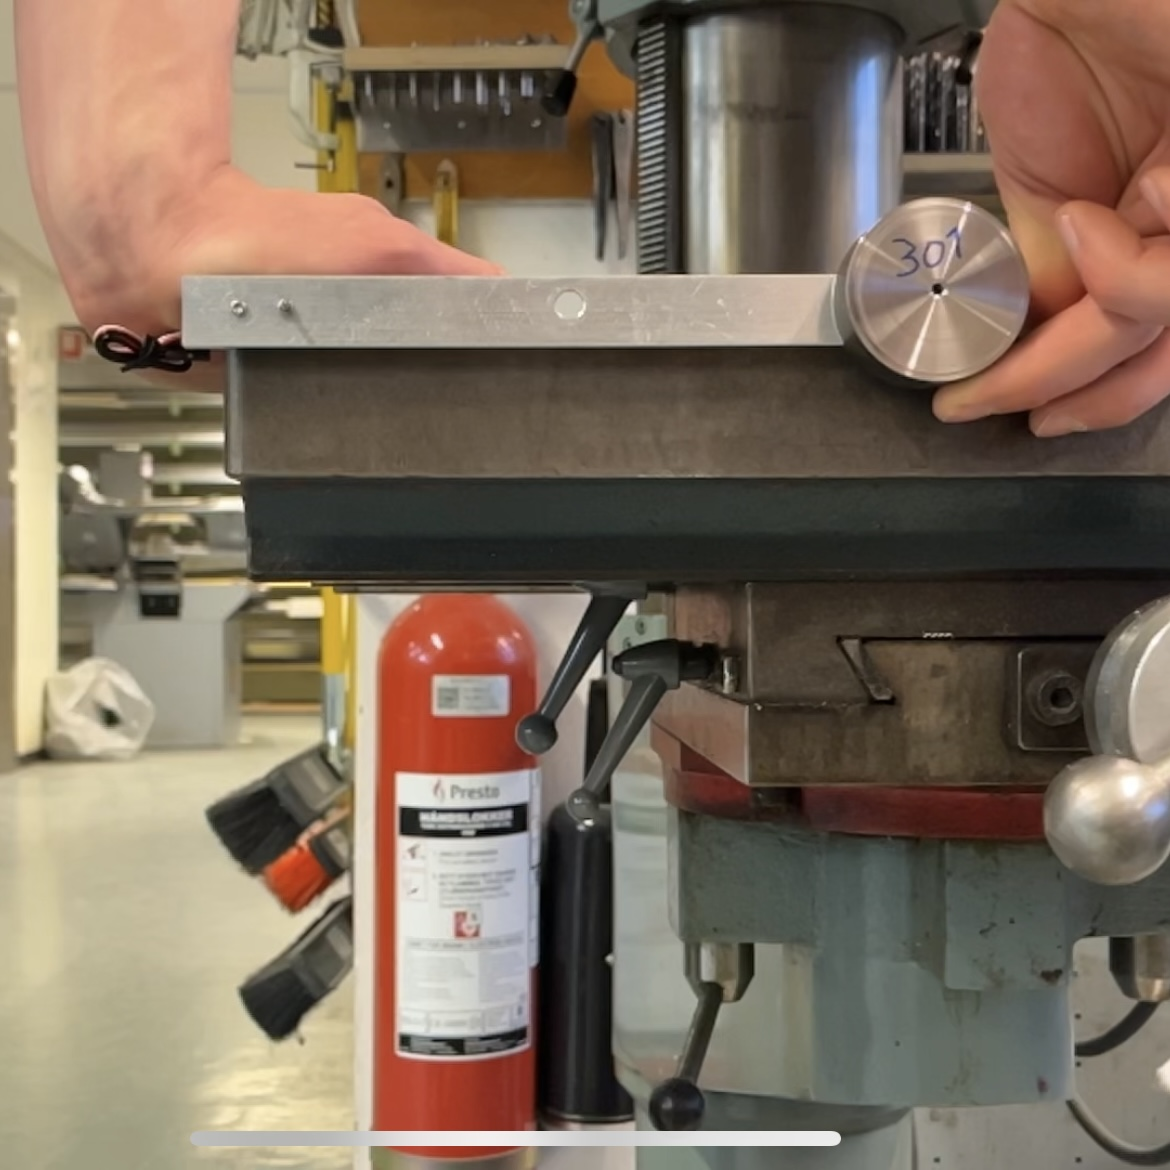
\includegraphics[width=0.6\textwidth]{Images/friction_estimation/big_motor.jpg}
    \caption{Experimental setup for motor friction estimation. An aluminum rod with ballast mass attached acts as a pendulum, with the motor shaft as the pivot point.}
    \label{fig:results:motor_friction_estimation:pendulum_setup}
\end{figure}

\subsection{Linear Regression Derivation}
Rearranging the equations of motion for linear regression:

\[
I \ddot{\theta} + \tau_{\text{gravity}} = -b_v \dot{\theta} - b_c \, \text{sign}(\dot{\theta})
\]

This can be expressed in matrix form:

\[
Y = X \beta
\]

where:
\begin{itemize}
    \item \( Y = -I \ddot{\theta} - \tau_{\text{gravity}} \),
    \item \( X = \begin{bmatrix} \dot{\theta} & \text{sign}(\dot{\theta}) \end{bmatrix} \),
    \item \( \beta = \begin{bmatrix} b_v \\ b_c \end{bmatrix} \).
\end{itemize}

The linear least squares solution for \( \beta \) is:

\[
\beta = (X^T X)^{-1} X^T Y
\]

This yields both the viscous damping coefficient \( b_v \) and the Coulomb damping coefficient \( b_c \).

To valiate the model we forward simulate the pendulum motion using the estimated parameters with a runge-kutta solver and compare the results with the measured data. This and the results are shown in section \ref{sec:results:motor_friction_estimation}.
